\chapter{Implementation Plan} 

\section{Schedule(Gantt-Chart)}

\begin{figure}[h]
    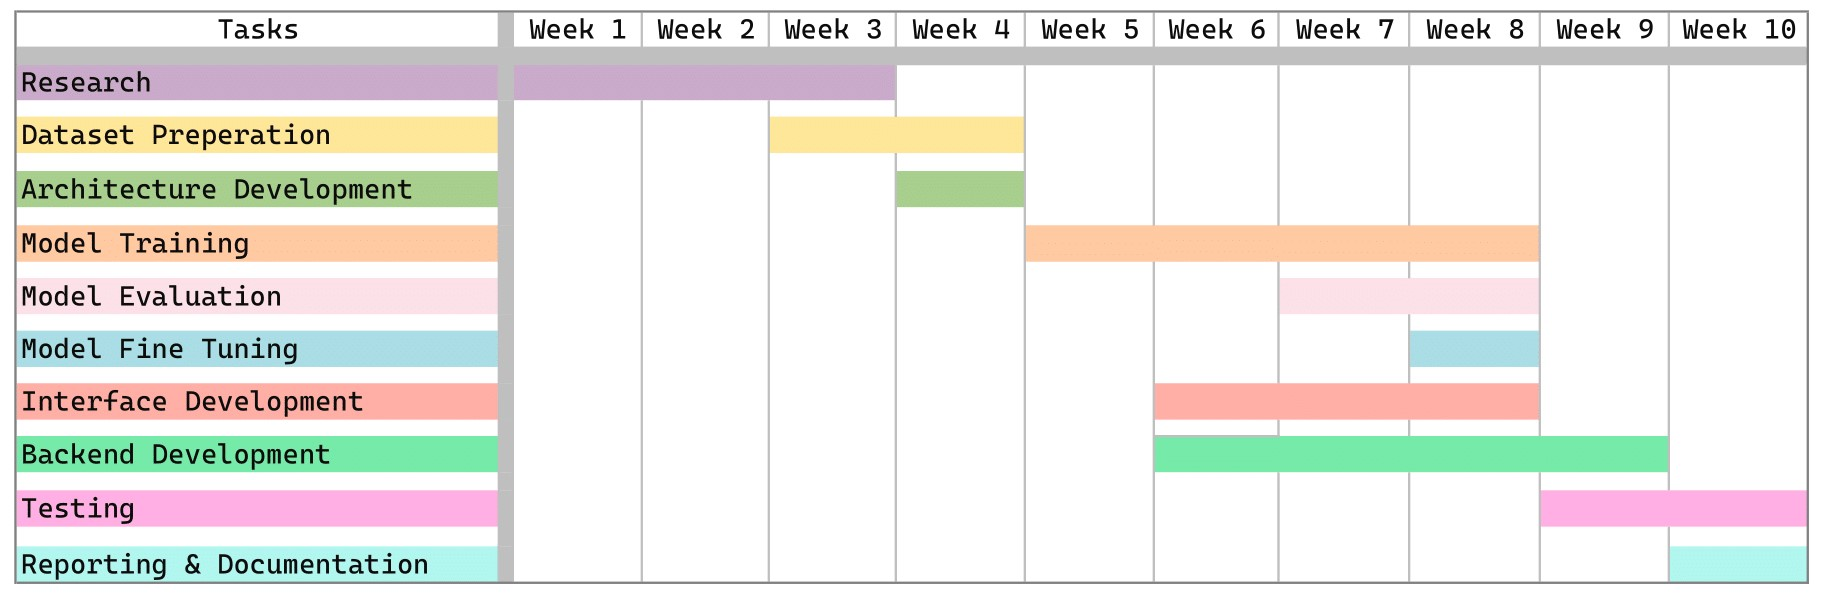
\includegraphics[width=15cm]{Image/Gantt-Chart.jpg}
    \caption{Gantt Chart}
\end{figure}
                
\section{SOFTWARE REQUIREMENT}
Our Facial Regonition   system requires Python, OpenCV, MySQL, TensorFlow, Flask,
CNN, JavaScript, Keras which are described below;
            \subsection{Python}
Python is a high-level interpreted programming language for general-purpose
programming created by Guido van Rossum which as released in 1991. Python has
design philosophy that emphasizes code readability, notably using significant white
spaces.The programming language features dynamic type system and automatic memory
management with support to multiple programming paradigms including Object
Oriented Imperative, Functional and Procedural. The programming language has large
comprehensive standard library.
\subsection{OpenCV (Open Source Computer Vision Library)}
OpenCV is a popular open-source library designed for computer vision tasks. It provides a wide range of functions and algorithms related to image and video processing.OpenCV is widely used for tasks like image and video processing, object detection, facial recognition, and more.
It is written in C++ but has Python bindings, making it accessible to a broader audience. 
\subsection{MySQL}
MySQL is an open-source relational database management system (RDBMS). Its name
is a combination of "My", the name of co-founder Michael Widenius's daughter, and
"SQL", the abbreviation for Structured Query Language. In our project, we use this
database to feed into PHP system for data labeling. The database is created from
scraping Nepali Sentiment text in python.
            \subsection{Tensor Flow}
TensorFlow is an open-source deep learning framework developed by the Google Brain team. It is widely used for building and training machine learning and deep learning models.It provides Flexible architecture for building various machine learning models.It supports deep learning, including neural networks and convolutional neural networks (CNNs).TensorFlow is used for developing and training deep learning models for tasks such as image classification, object detection, natural language processing, and more.
   \section{FUNCTIONAL REQUIREMENT}
\subsection{Face Detection}
Accurate face detection algorithms should be implemented to identify and locate faces in images or video streams.
\subsection{Face Recognition}
Employ robust facial recognition algorithms for accurate identification of registered individuals.
The system should provide a confidence score or percentage to indicate the level of certainty in the recognition process.
\subsection{Database Management}
The system should manage a secure database of people data and their corresponding facial features.
Allow easy addition, modification, or removal of people from the database.

\subsection{Real-time Monitoring}
Provide real-time monitoring capabilities for administrators.

 \section{NON-FUNCTIONAL REQUIREMENT}
These requirements are not needed by the system but are essential for the better
performance of sentiment engine. The points below focus on the non-functional
requirement of the system.
           \subsection{Performance}
\subsubsection{Response Time} The system should have low latency in recognizing faces and tracking recognized person.
\subsubsection{Throughput} It should be able to handle a specified number of facial recognition and tracking.
\subsection{Scalabiity}
The system should be scalable to accommodate an increasing number of people.
\subsection{Reliability}
The system should be highly reliable, minimizing the risk of false positives or negatives in facial recognition.
It should have mechanisms to handle system failures and recover gracefully.
\subsection{Availability}
The system should have a high level of availability to ensure that it is accessible when needed.
\subsection{Security}
\subsubsection{Data Security} Facial data should be stored and transmitted securely, following industry best practices.
\subsubsection{Access Control}Implement robust access control mechanisms to restrict unauthorized access to the system.